%!TEX root = ../thesis.tex
\chapter{Results}
\label{ch:results}

In this chapter we present the results we compiled during the course of our work.
This includes an evaluation of the developed hexapod model and its locomotion controller, as well as review of the RL training results obtained and lessons learned from observing the training process.

\section{Evaluation: Hexapod model}
During the development process of the hexapod model and locomotion controller, we observed that the conceived model architecture enables us to quickly modify and/or add components.
An example of this flexibility is provided by the retrospective addition of sensor readings for the rotational acceleration of the \textalpha-joints.
As the hexapod leg is defined as a library component, it was only necessary to enable the respective sensor reading one the joint block and add the new signal to the already existing sensory information bus. 
There was no need to modify the hexapods legs individually, as Simulink automatically updates all library-linked blocks.
In general, the library of custom subsystems has proven to be a most useful tool, reducing development time and promoting modularity.
The encapsulation of the hexapod model as a whole into a single, top-level subsystem block, that only reveals necessary in- and outputs, provides the developer with a simple to understand interface.
It also gives us the ability to duplicate the complete hexapod system without any effort, which could prove useful in future research as it enables the system to easily be utilized in multi-agent simulations.

Concerning the actual simulation of the model, it can be said that in most cases where the robot uses a statically defined gait pattern for locomotion, a simulation step size of 0.5 ms yields stable results and runs at close to real time.
Given an untrained, exploring RL agent as the models operator, a step size of 0.25 ms is preferable, as sudden twitching and jerking motions might occur, which can lead to simulation instabilities and exceptions.
Similar to the results of \cite{thilderkvist2015motion}, we begin to observe these simulation problems at larger step sizes ($> 0.5 ms$), although not of the same significance and frequency as described by them. 
The most common reason for exceptions we observed, were collision detection failures.
These occur, when two rigid bodies move into each other faster than the simulation solver can observe, due to its limited temporal resolution.
During the several ten-thousand simulation episodes performed at a step-size of 0.25 ms during RL training, we did not once observe am exception.
Overall, the behaviour of our robot model seems, to the best of our knowledge, but without the co-examination of a real world counterpart, physically accurate.


We attribute the unsatisfactory results \cite{thilderkvist2015motion} experienced from the spatial friction forces to be most likely linked to deciding on a step size too large for stable simulations.
As they also work with an earlier MATLAB version, using Simscape's predecessor \textit{SimMechanics}, the problems might also have arisen from a possibly more primitive physics model.

To summarize, we were able to create a well-functioning, virtual model of a hexapod robot.
Simulations of the model are robust and physically accurate
We are confident that the model can serve as a platform for future research as it utilizes a modular architecture, can easily be expanded and is based on the versatile MATLAB environment.
 

\section{Evaluation: Locomotion Controller}
The locomotion controller we presented in \ref{subsec: Locomotion controller} is the result of several design iterations.
We extensively tested each of the designs to uncover their weakpoints, upon which the next iteration was improved on.

The initial design (\textit{MK1}) enabled the robot to walk in a straight line tripod gait.
We observed that the hexapod model, controlled by MK1, would jerk up and down significantly during a movement cycle, as can be seen in \hyperref[vid: MK1]{MK1} and \ref{figure: Thorax Height graph, bad tuning}.
During a legs swing phase, the robots thorax would slowly sink towards the side of the lifted leg and be rapidly pushed upwards again at the end of the swing.
As we defined the trajectory relative the thorax and did not consider sensing ground contact, the leg on the sinking side would hit the ground earlier than expected by the controller, as the anticipated AEP "sunk" into the ground plane.
We were able to later on attribute this behaviour to the slow reactions of the PID controllers.
These were, given our initial tuning parameters ($K_p = 3, K_i = 0.2, K_d = 1, N = 100$), unable to follow their assigned trajectories. 
In addition, the MK1 controller version requires a lot of calculation time per simulation step, resulting in high simulation times.
The observed cause of the being the computationally intensive, iterative IK block provided by Simulink, as we have already elaborated on in \ref{subsubsec: IK Solver}.

With the subsequent version, \textit{MK2}, we focused on introducing tetrapod and wave gait as well as increasing simulation speed.
Implementing the gait patters proved to be straightforward, as, resulting from the models modular architecture, solely the leg coordination of the static gait definition had to be modified.
The resulting simulations of the robot walking in tetrapod and wave gait can be observed in \hyperref[vid: MK1]{MK2}.

The decision to implement our own, custom analytical IK solver resulted in a significant performance boost.
Comparing the MK1 and MK2 controllers, we are able to achieve an up to 10x speed up in simulation time.
\todo{Prove with a comparison of MK1 and MK2 simulation time}

With the final non-RL controller design, termed \textit{MK3}, we improved the stability of the hexapods locomotion as well as introduced the capability for omnidirectional movement.
By simply re-tuning the PID controller parameter to the values displayed in \ref{table: PID parameters}, we were able to reduce the jerking behaviour of the robot far enough to not be visually noticeable.
A comparison of the thorax's height differences during movement, when under control of the MK2 and MK3 controllers, can be seen in Fig. \hyperref[vid: MK1]{MK3}.

\begin{figure}[h]
	\begin{subfigure}{\textwidth} % this sets the figure to be max half the width of the page
		\centering
		% include first image
		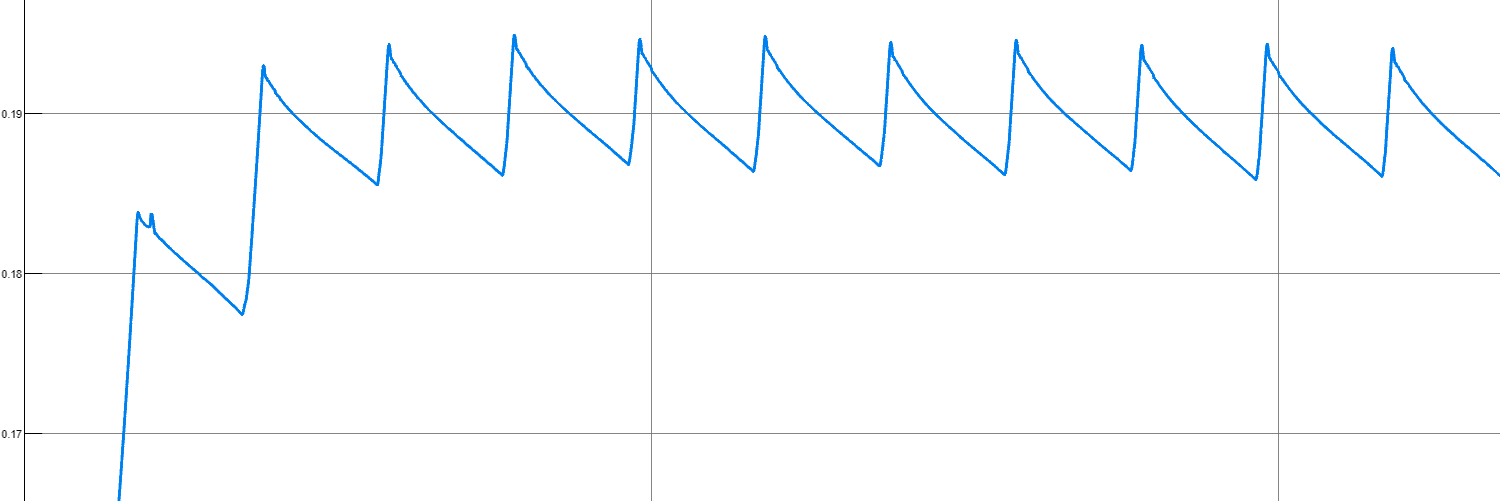
\includegraphics[width=\linewidth]{ThoraxHeight_firstPID.PNG}  % this sets the image to fill 90% of the available space -> 45% of the line width in total. 
		\caption{}
		\label{figure: Thorax Height graph, bad tuning}
	\end{subfigure}
	
	\begin{subfigure}{\textwidth}
		\centering
		% include third image
		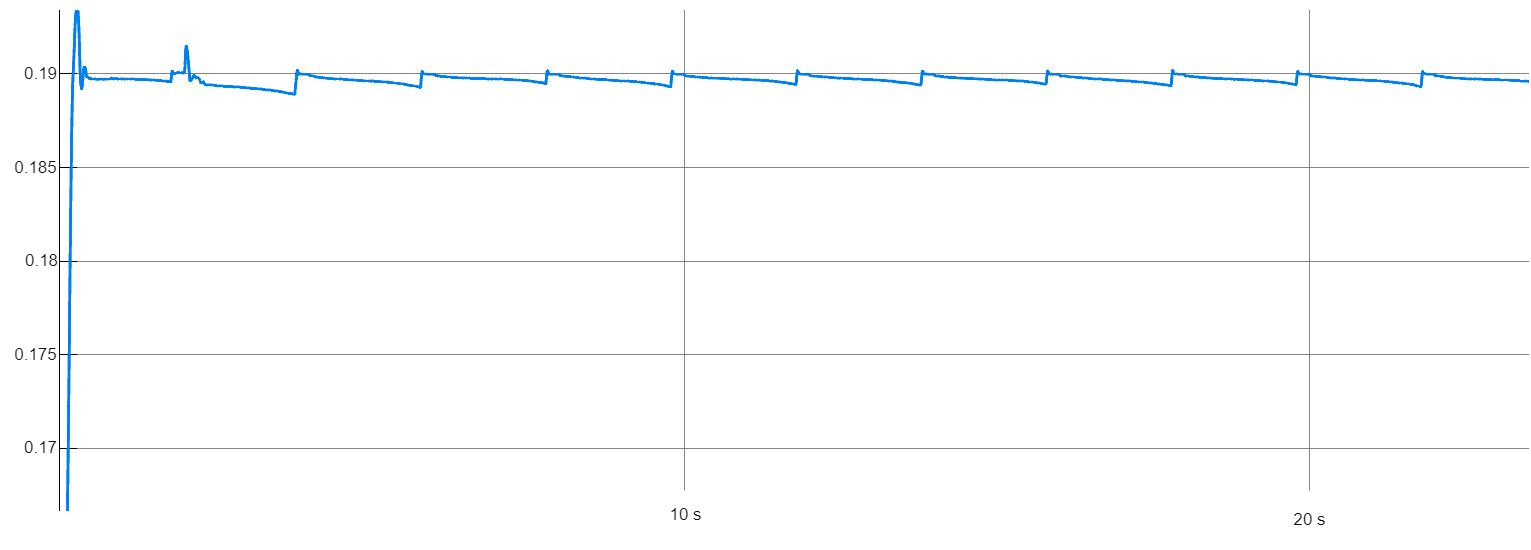
\includegraphics[width=\linewidth]{ThoraxHeight_retunedPID.PNG}   % this width should be half of the width of the other two images
		\caption{}
		\label{figure: Thorax height graph, re-tuning}
	\end{subfigure}
	\caption[Thorax height graphs]{(a) Thorax height graphs of hexapod robot controlled by (a) MK2 and (b) MK3 controller.}
	\label{figure: Thorax height graphs}
\end{figure}



\todo{major rewrite and update}
\section{Evaluation: RL training}
In this section, we present the result obtained during training RL agents on the problem of leg coordination.
We begin with an evaluation of the overall process, after which we separately present the training results of the DDPG an PPO agents.

Implementing a RL agent yielding satisfying results proved to be more difficult than anticipated.
As there exists a large set of parameter to be considered during setup, finding a set of well-working parameters is a time-consuming task.
This is reinforced by the fact that, to observe the performance of a set of parameters, we found the agent needed to train for at least 1-2k episodes, equating to several hours of runtime given the hardware used.
Additionally, as we ran experiments with two different RL algorithms, we were required to tune two separate sets of parameters.

In total, we ran over 20 documented agent configurations, each with a different set of parameters.
As we are not able to present all of the results here, a 
The parameters common to both algorithms are presented in table \ref{}.

\subsection{Reward Exploitation}
A problem often observed in RL is an agent exploiting a poorly-defined reward function.
This commonly leads to agents exhibiting undesirable behaviour, even though according to the reward function they are performing well.

{\def\arraystretch{1.4}\tabcolsep=5pt
	
\begin{table}
	\parbox{.4\linewidth}{
		\centering
		\begin{tabular}{| c | c |} 
		\hline
		\textbf{Training params.s} & \textbf{Value} \\ [0.5ex] 
		\hline
		\hline
		Sample time & 0.05 s \\ 
		
		Episode steps & 512 \\
		
		\hline
		\textbf{Agent params.} &  \\ [0.5ex] 
		\hline
		
		Learn Rate & $\num{3e-4}$ \\
		
		Episode steps & 512 \\
		
		Exp. Buf. length & $\num{1e6}$ \\
		
		Discount factor &  0.99 \\
		
		Mini-Batch size & 32 \\
		
		NN-width & 128 \\
		
		\hline
		\textbf{Noise params.} &  \\ [0.5ex] 
		\hline
		
		\textsigma\footnote{\textsigma: Standard Deviation} & 0.05 \\
		
		\textsigma-decay\footnote{\textsigma-decay: Decay rate of \textsigma. Each sample time step k, \textsigma decays according to following formula: $\sigma_{k+1} = \sigma_k \cdot (1 - \textbf{\textsigma-decay})$} & 1e-6 \\
		
		\hline
	\end{tabular}	
	\caption[DDPG agent parameters]{}
	\label{table:DDPG parameters}
	}
	
	%\hfill
	
	\parbox{.4\linewidth}{
		\centering
		\begin{tabular}{| c | c |} 
		\hline
		\textbf{Training params.} & \textbf{Value} \\ [0.5ex] 
		\hline
		\hline
		Sample time & 0.05 s \\ 
		
		Episode steps & 512 \\
		
		\hline
		\textbf{Agent params.} &  \\ [0.5ex] 
		\hline
		
		Learn Rate & $\num{3e-4}$ \\
		
		Episode steps & 512 \\
		
		Exp. Buf. length & $\num{1e6}$ \\
		
		Discount factor &  0.99 \\
		
		Mini-Batch size & 32 \\
		
		NN-width & 128 \\
		
		\hline
		\textbf{Noise params.} &  \\ [0.5ex] 
		\hline
		
		dev (\textsigma) & 0.05 \\
		
		devdec & 1e-6 \\
		
		\hline
		\end{tabular}
		\caption[PPO agent parameters]{}
		\label{table:PPO parameters}
	}
\end{table}
}

{\def\arraystretch{1.4}\tabcolsep=5pt
\begin{table}
	\centering
	\begin{tabular}{| c | c |}
		\hline
		\textbf{Weight} & \textbf{Value}\\
		\hline
		\hline
		$c_{s_x}$   		&  1	\\
		$c_{v_x}$   	    &  50	\\
	  	$c_{v_y}$  		    &  1	\\
	  	$\Delta_h$  		&  1	\\
	  	$c_W$ 				&  0.025\\
		\hline
	\end{tabular}
	\caption[Reward weights]{}
	\label{table: Reward weights}
\end{table}
}

The survival reward $r_\text{survival}$ is set at 0.1, resulting in the agent receiving $0.1 \cdot 512 = 51.2$ cumulative reward during a full episode.


We used the \textbf{D}eep \textbf{D}eterministic \textbf{P}olicy \textbf{G}radient (DDPG) algorithm, an actor-critic, model-free, online, off-policy RL method.
The actor network consists of a 12-wide observation input layer followed by 3 100 neuron wide fully-connected layer, in between each of them a ReLU-layer to introduce non-linearity.
Concluding the actor network is an output layer consisting of 6 neurons, one for each action channel.
The architecture of critic network is more complicated, as it has to take in more informations.
At the start this network consists of two separate branches, one taking as inputs X and one Y.
On both branches the input layers are followed by a fully-connected and a ReLU layer.
At this point the two branches are connected by a simple addition layer.
After the add-layer, another 2 combinations of fully-connected and ReLU layer follow, concluding with a single output neuron, representing the critics reward estimation.
All of the actor and critic layers are, if not mentioned otherwise, 100 neurons wide.
The architectures of the actor and critic networks have been adopted from example applications created by \cite{matlabDDPGExample, matlabPPOExample}.

We used a learning rate of $3e^{-4}$ and $1e^{-3}$ for the actor and critic respectively and a discount factor of 0.99.
The agents sample rate is set at 0.05, meaning the agent samples the environment and takes an action every 50 ms.
A more detailed summary of the RL parameters is given in table \ref{table: DDPG parameters}.

{\def\arraystretch{1.4}\tabcolsep=5pt
\begin{table}
	\centering
	\begin{tabular}{| l | c |}
		\hline
		\textbf{Parameter} & \textbf{Value}\\
		\hline
		\hline
		Actor learn rate & $3e^{-4}$ \\
		Critic learn rate & $1e^{-3}$ \\
		Discount factor &  0.99 \\
		Mini-Batch-Size & 16 \\
		Experience buffer & $1e^6$\\
		\textsigma \ (UB) & 0.2 \\
		\textsigma-decay (UB) & $1e^{-6}$ \\
		
		\hline
	\end{tabular}
	\caption[DDPG parameters]{DDPG parameters. Uhlstein-Beck (UB) noise model is used to introduce noise into the agents exploration}
	\label{table: DDPG parameters}
\end{table}
}


\begin{figure}[h]
	\begin{subfigure}{\textwidth} % this sets the figure to be max half the width of the page
		\centering
		% include first image
		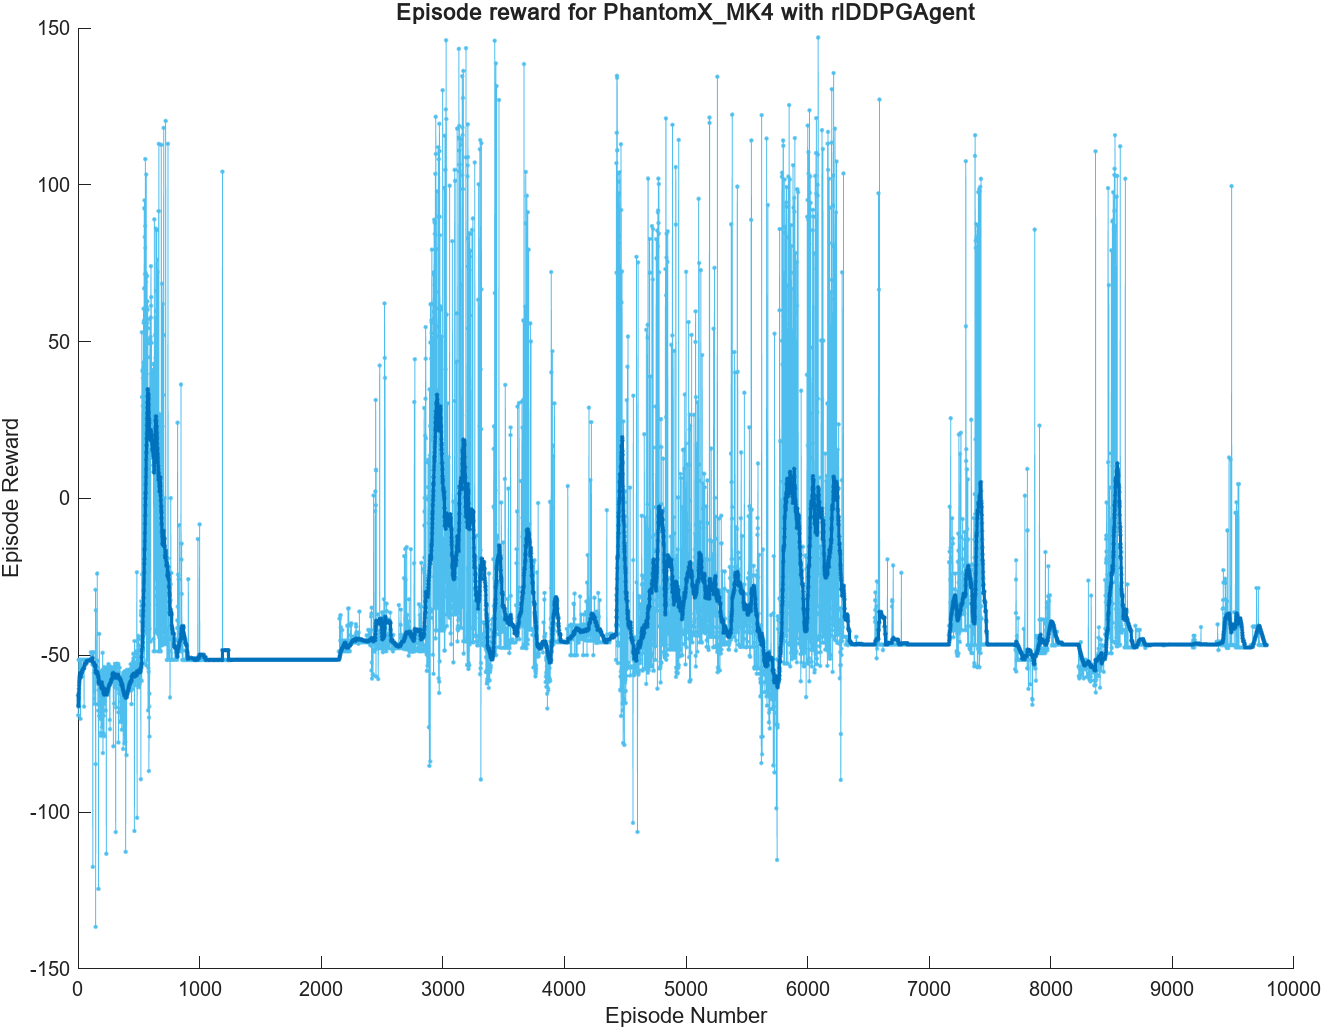
\includegraphics[width=\linewidth]{graphs/firstSuccess_146reward}  % this sets the image to fill 90% of the available space -> 45% of the line width in total. 
		\caption{}
		\label{figure: RL a}
	\end{subfigure}
	\begin{subfigure}{\textwidth}
		\centering
		% include second image
		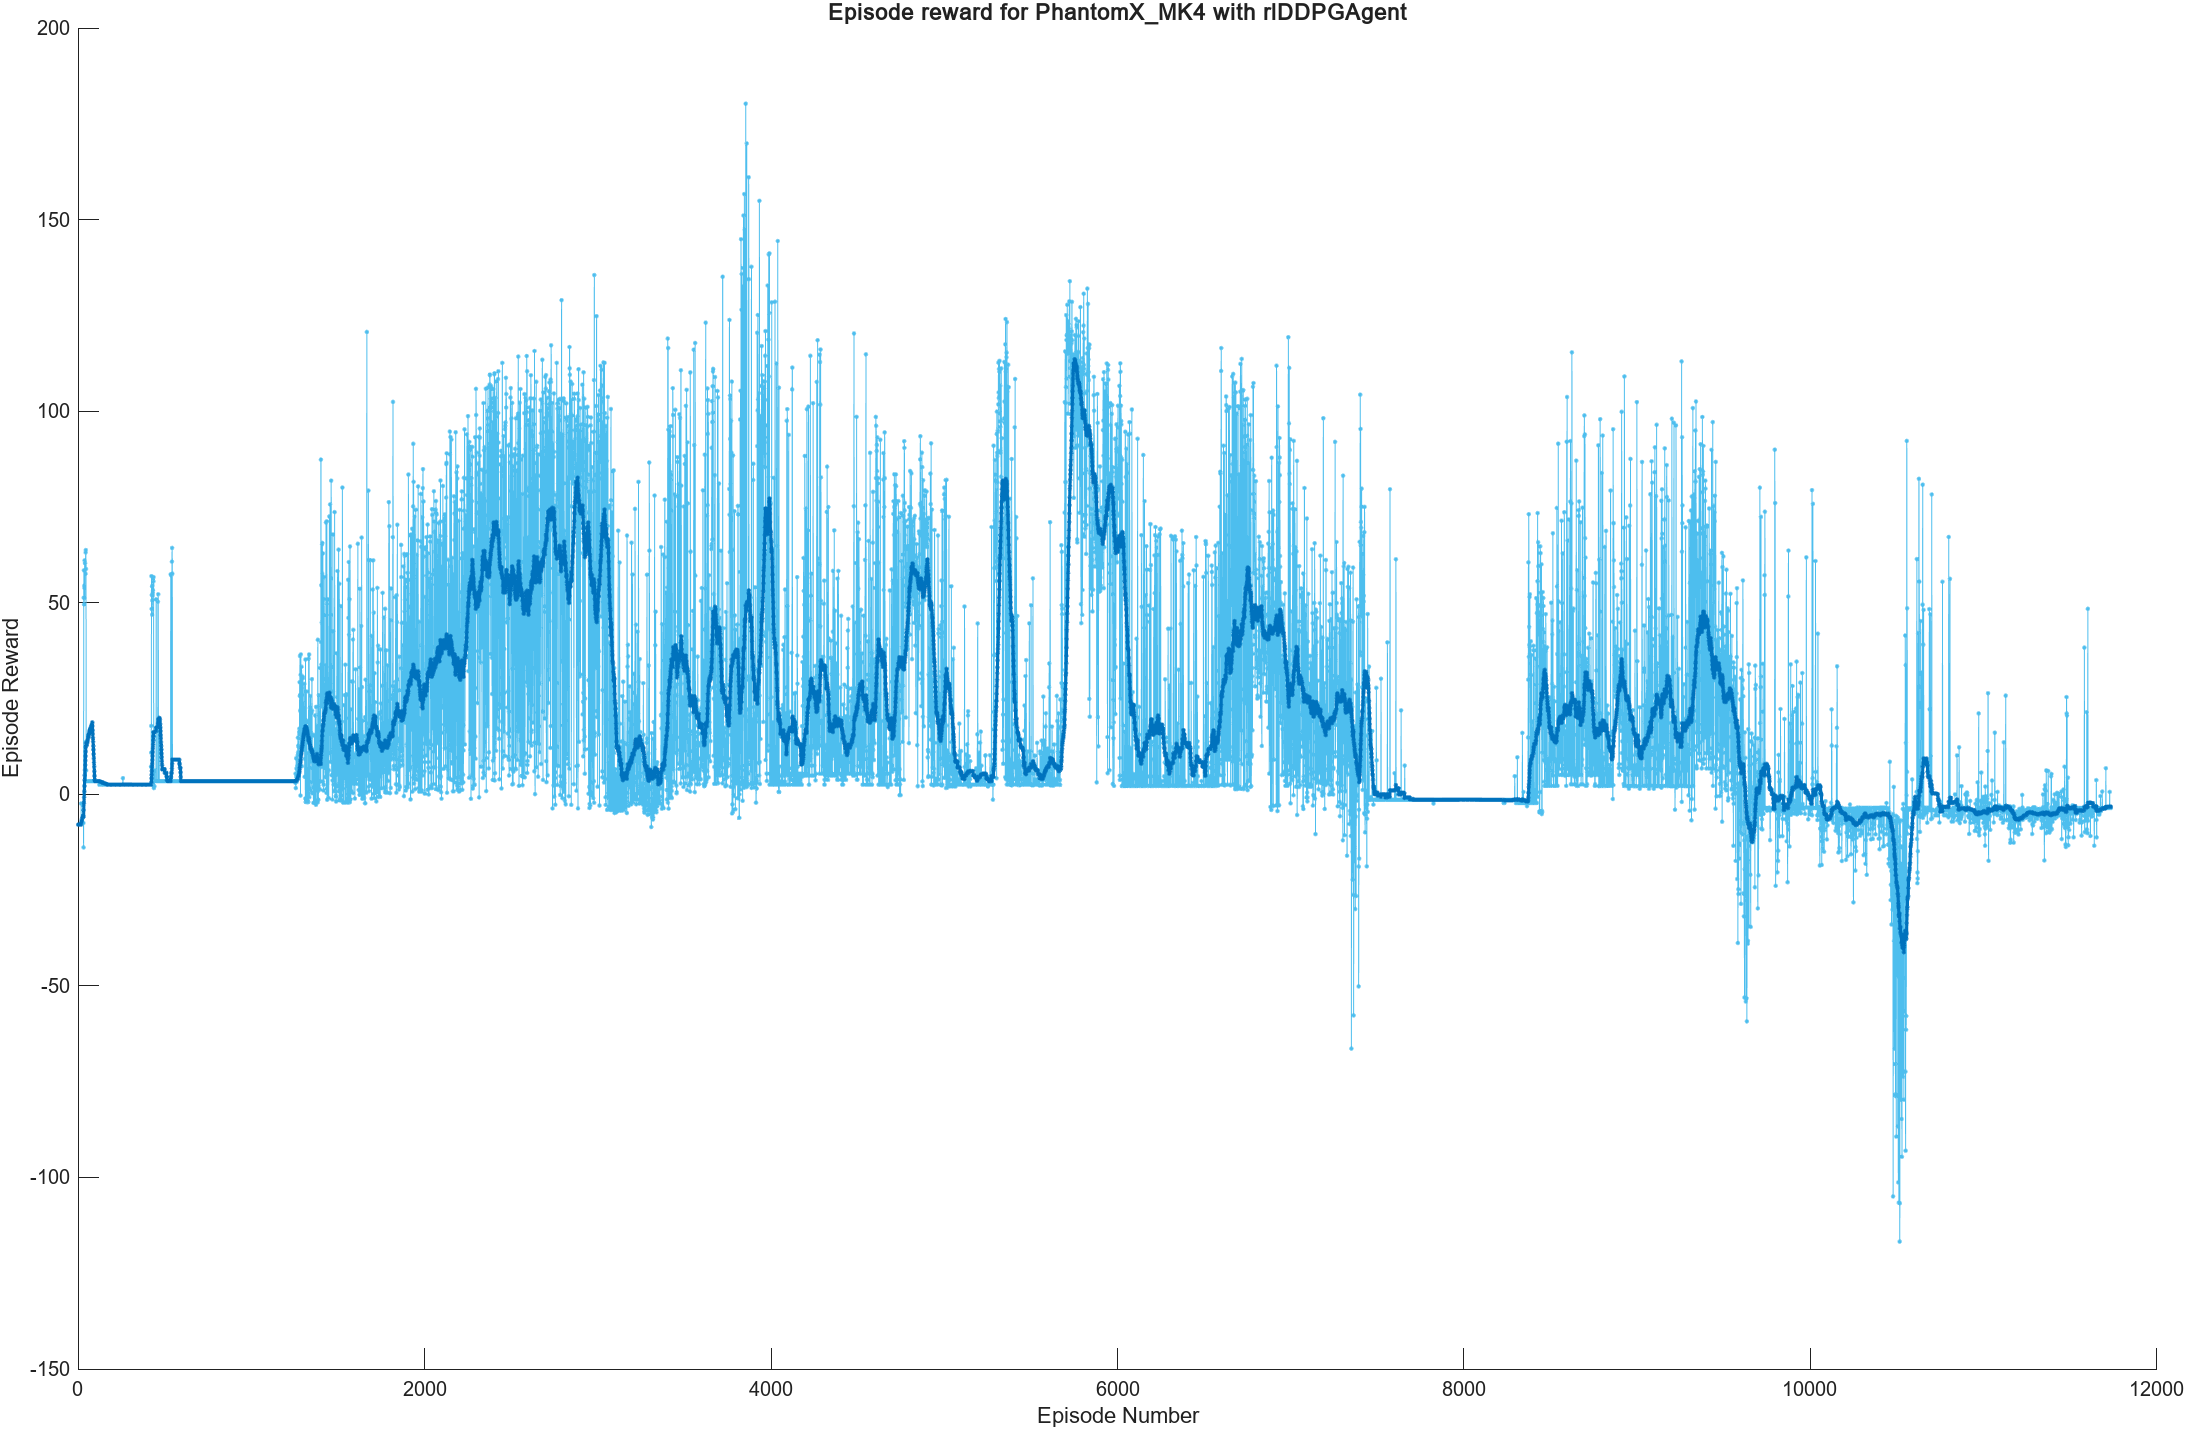
\includegraphics[width=\linewidth]{graphs/DDPG_reward_180.PNG}  
		\caption{}
		\label{figure: RL b}
	\end{subfigure} 
		\caption[DDPG training graphs (1)]{DDPG training graphs (1). (a) first Success 146. (b) DDPG Reward 180.}
	\label{figure: DDPG learning graphs 1}
\end{figure}

\begin{figure}[h]
	\begin{subfigure}{\textwidth} % this sets the figure to be max half the width of the page
		\centering
		% include first image
		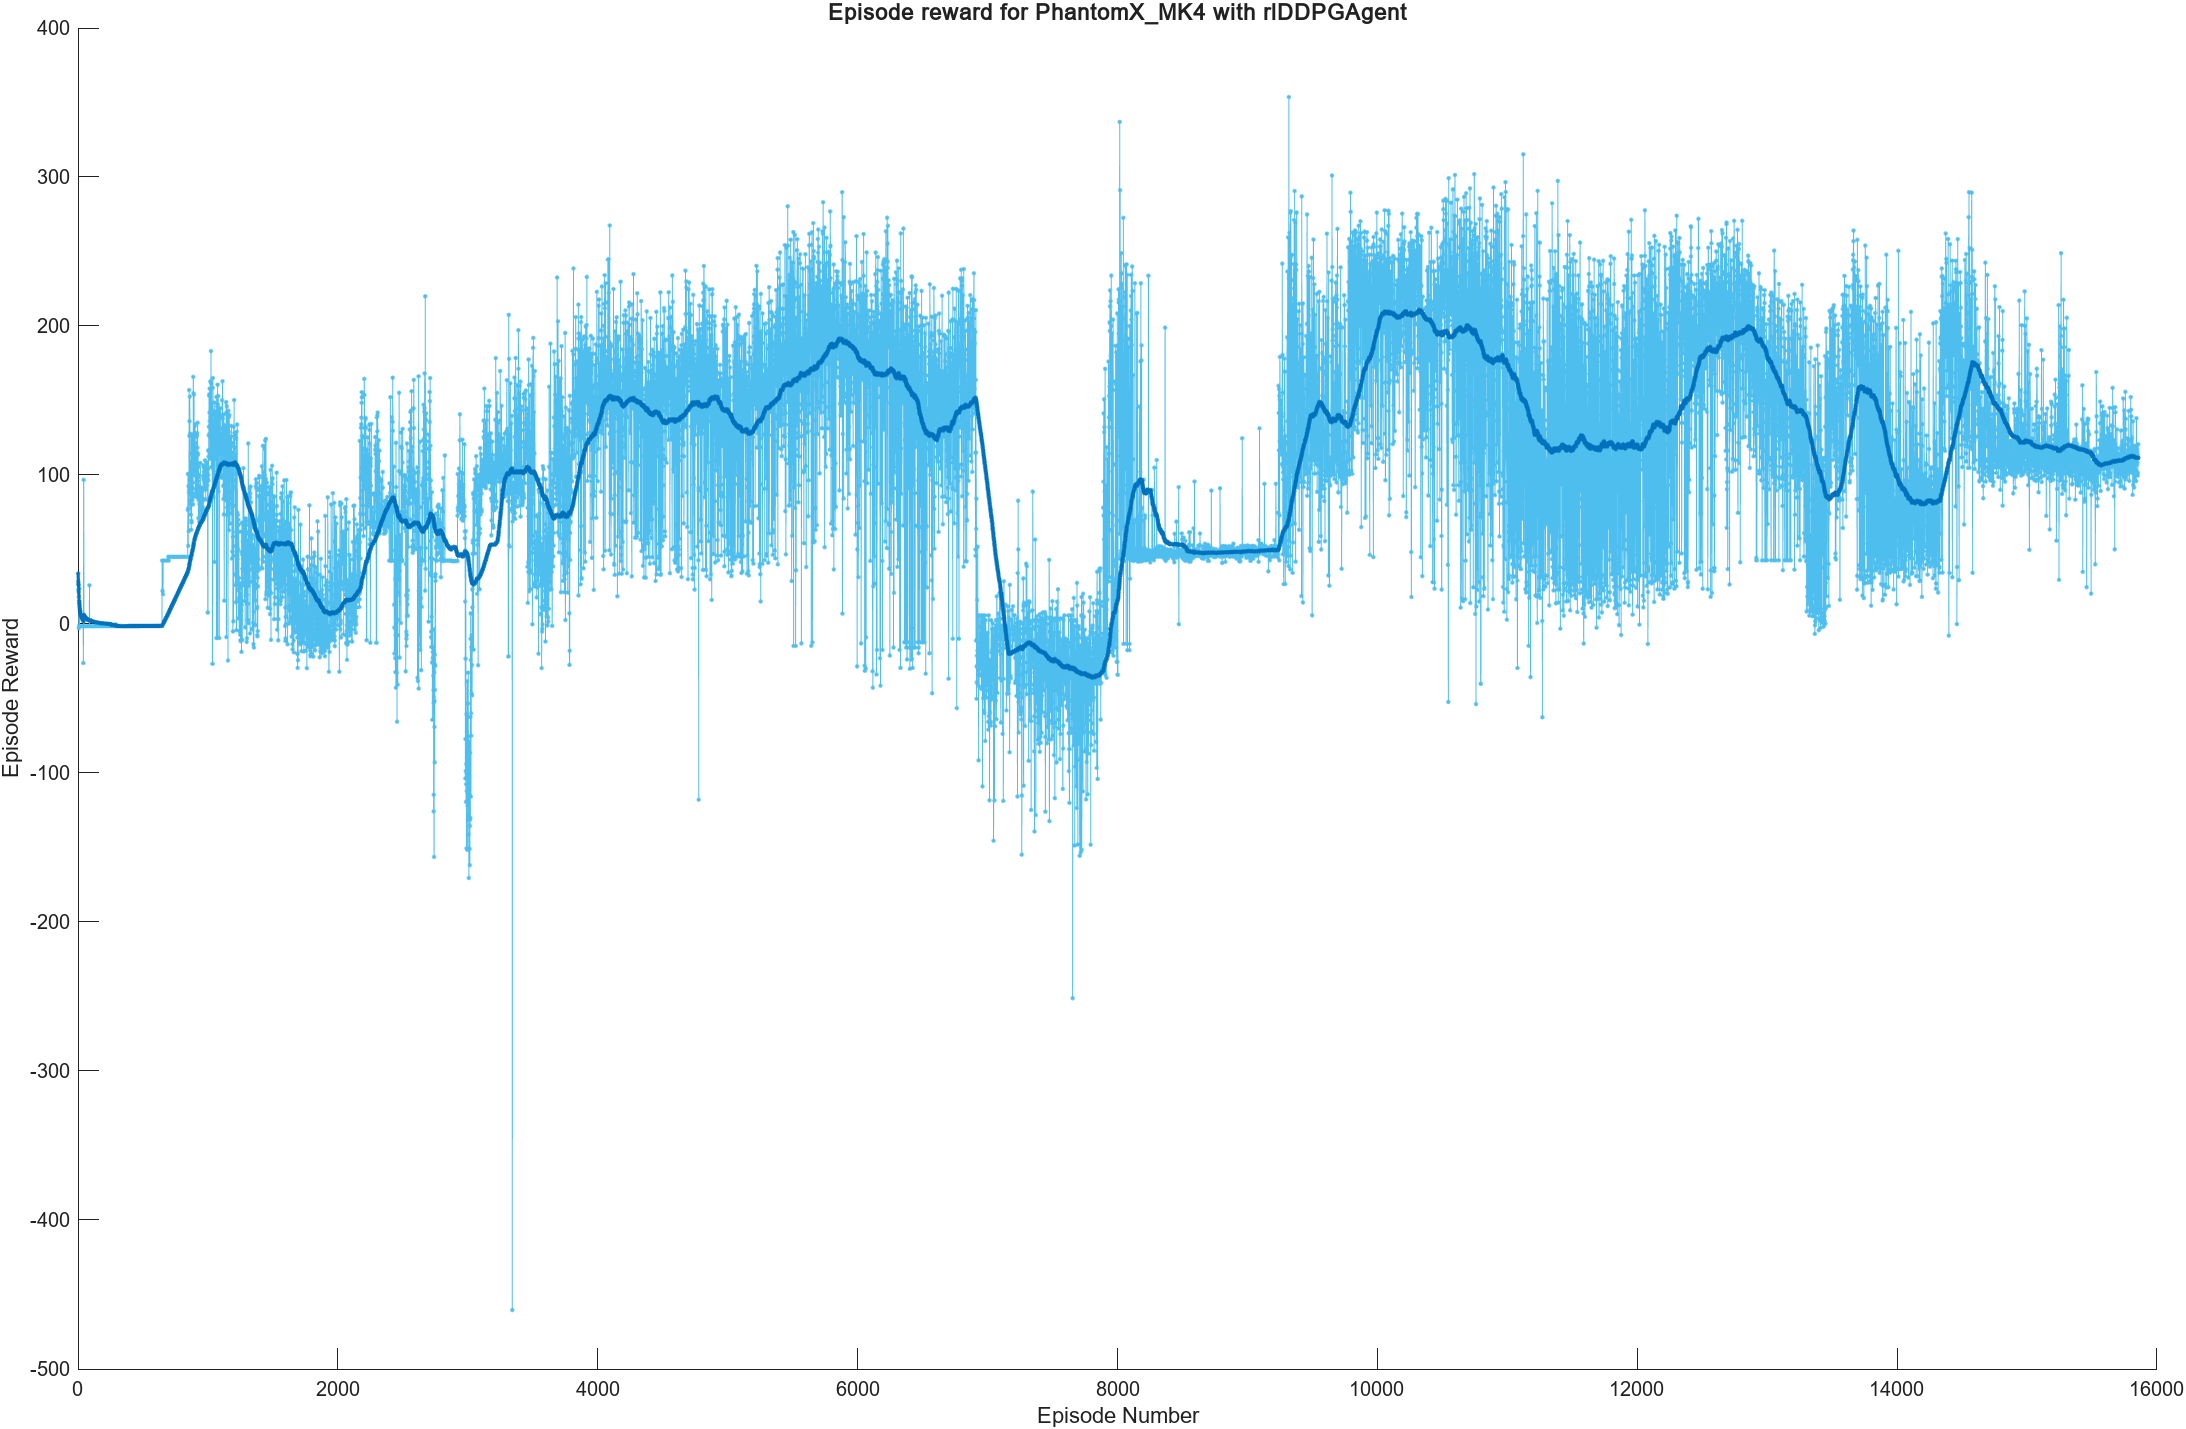
\includegraphics[width=\linewidth]{graphs/redefinedReward_50x_vx.PNG}  % this sets the image to fill 90% of the available space -> 45% of the line width in total. 
		\caption{}
		\label{figure: RL c}
	\end{subfigure}
	\begin{subfigure}{\textwidth}
		\centering
		% include second image
		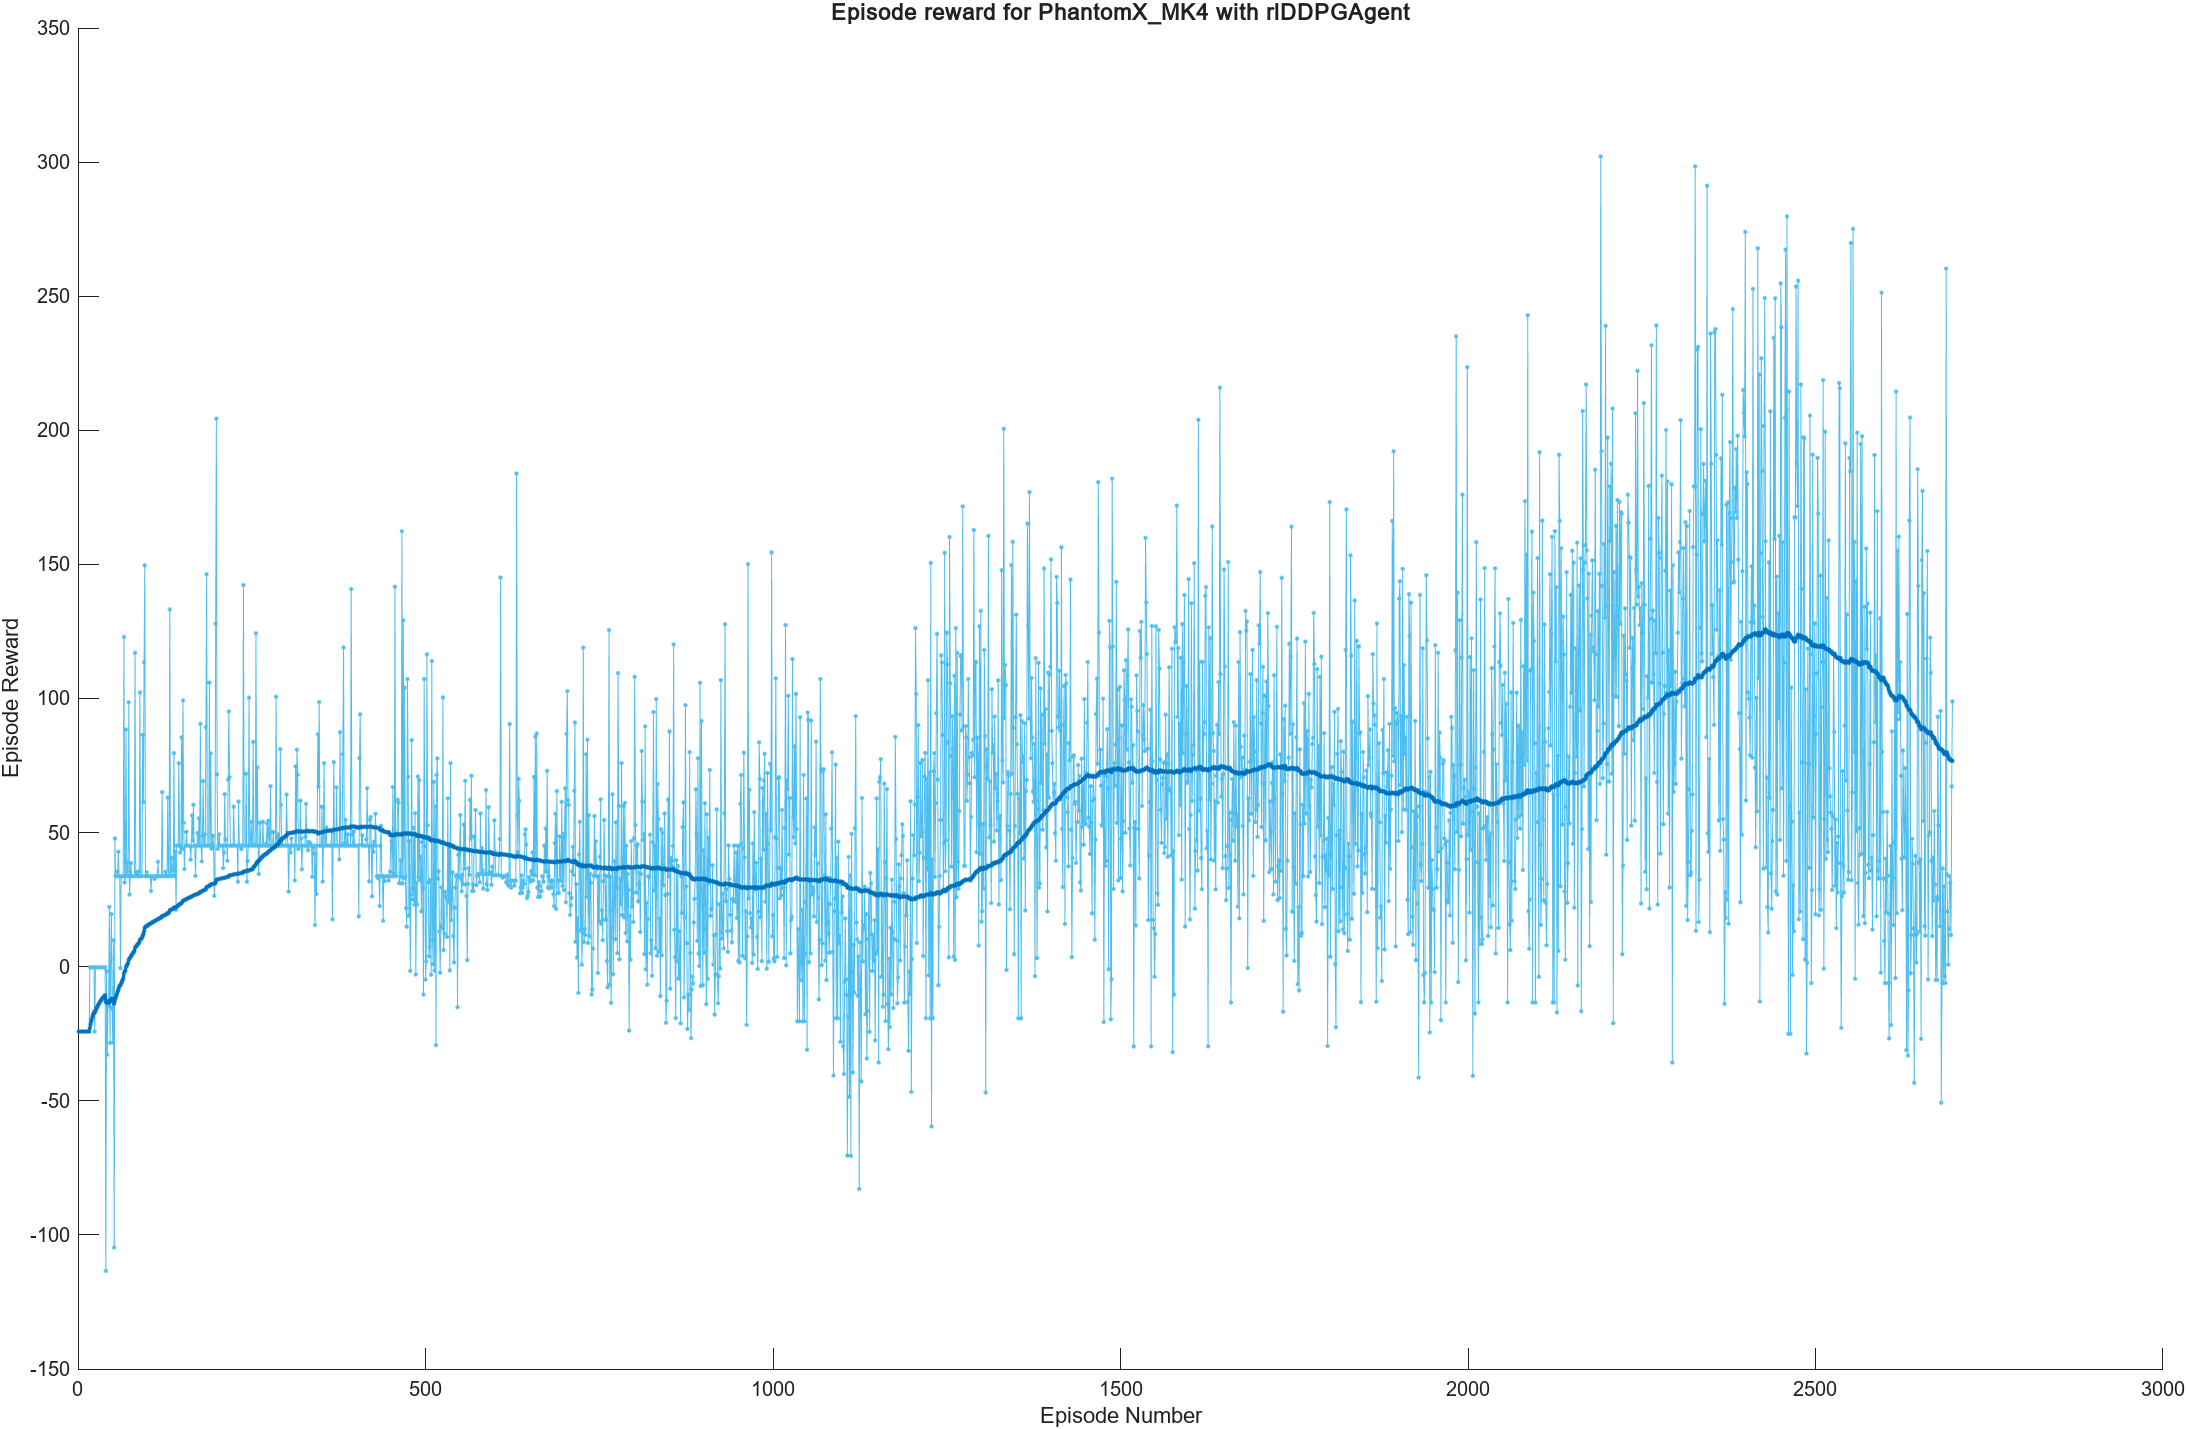
\includegraphics[width=\linewidth]{graphs/lastAgent_graph}  
		\caption{}
		\label{figure: RL d}
	\end{subfigure} 
	\caption[DDPG training graphs (2)]{DDPG training graphs (2).  (a) redefined Reward 50x vx. (b) lastAgent.}
	\label{figure: DDPG learning graphs 2}
\end{figure}



When we first started working on the RL process, te result were not very promising. The agent did stabilize, meaning it did not jump around randomly, but it was not able to find an efficient gain.
The agent never learned to reliably move a leg forward if it was starting to drag behind due to reaching the PEP.

Early on in the RL setup process we realized that the current inputs into the hexapod model are not suitable for reinforcement learning.
These initial inputs, frequency, duty cycle and offsets were better suited to being statically optimized instead of learned.
The new inputs, one signal per leg to initiate the swing phase, are much more suited for RL, as they enable a more complex and dynamic interaction with the robot.
Only after implementing these changes were we able to record the first successes in learning.


\textit{MATLABs Parallel Computing Toolbox} provided a significant boost in learning performance.
By being able to run 8-16 agents in parallel , one per processor core or multiple in separate threads, we were able to speed up the learning process significantly.
This allowed us to test several different agent configurations in an acceptable amount of time and also enabled us to refine well performing agents by running more episodes.

The simulation studies and RL training we run in this work are accomplished with a desktop computer powered by an Intel i7-11700K CPU, 32 GB of RAM and a NVIDIA RTX 2060 GPU.

Concerning MATLAB, we used the version 2023a for all of our work.


The final, successful agent trained for x episodes and a total of x simulation steps. 
This means the agent trained for about x hours of real time to achieve the results.

We are confident that, given more time to carefully tune parameters and reward, the training time could be reduced significantly and performance improved.

